%!TEX root = ../eval1.tex

\exe{2, difficulty=1}{
	Soit $A(x;x)$ un point dépendant d'un paramètre réel $x\in\R$.
	
	Où se situe le point $A$ ? Placer ses positions possibles dans le repère ci-dessous.
	
	\begin{center}
	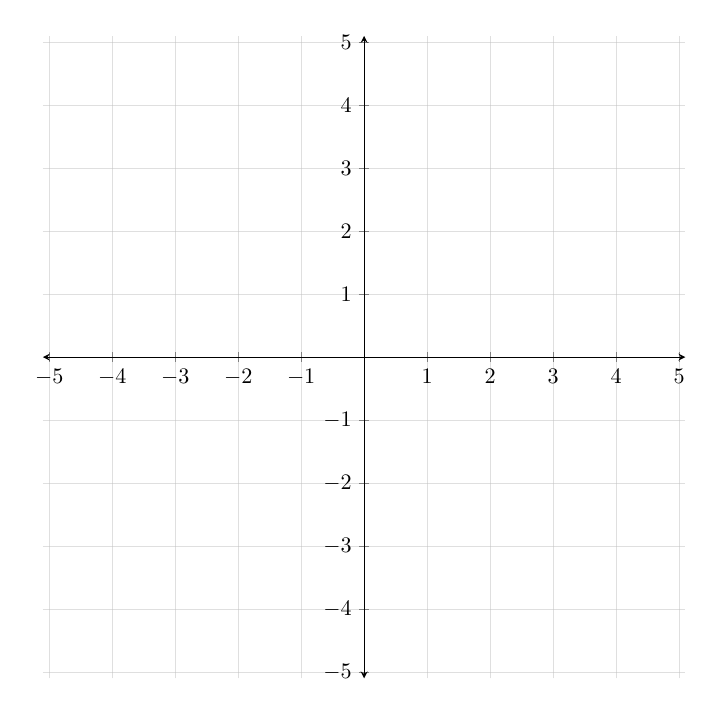
\begin{tikzpicture}[>=stealth, scale=.8]
		\begin{axis}[xmin = -5.1, xmax=5.1, ymin=-5.1, ymax=5.1, axis x line=middle, axis y line=middle, axis line style=<->, xlabel={}, ylabel={}, grid=both, grid style = {opacity=.5}, clip=false, xtick distance = 1, ytick distance=1, x=1cm, y=1cm]
		\end{axis}
	\end{tikzpicture}
	\end{center}
}{exe:diagonale}{

	On teste plusieurs valeurs de $x\in\R$, sans oublier des valeurs négatives ou non entières.
	
	En plaçant les points $(1;1), (-3; -3), (2,1 ; 2,1), (-0,5 ; -05), \dots$, on remarque que les positions possibles de $A$ se situent sur la diagonale ci-dessous.
	
	\begin{center}
	\begin{tikzpicture}[>=stealth, scale=.7]
		\begin{axis}[xmin = -5.1, xmax=5.1, ymin=-5.1, ymax=5.1, axis x line=middle, axis y line=middle, axis line style=<->, xlabel={}, ylabel={}, grid=both, grid style = {opacity=.5}, clip=false, xtick distance = 1, ytick distance=1, x=1cm, y=1cm]
		\draw[BLUE_E, -, very thick] (axis cs:-5,-5) -- (axis cs:5,5);
		\end{axis}
	\end{tikzpicture}
	\end{center}
}